\chapter{Project results}
\textit{This chapter seeks to present the results from this project.}

A system of a CDU and two sensor nodes has been made. The CDU can communicate with the sensors notes using the custom power line communication bus. The sensor nodes can respond to all the defined function codes and if the addressed sensor receives an unknown function code it will respond with an error.\\
The data from the sensor node is received by the CDU and stored in memory. This can be exported to a PC by requesting data from the CDU.\\
The sensor nodes can measure temperature.
\section{CDU}
The CDU prototype has memory, pc communication, sensor communication, sensor power supply and power supply fully implemented. The µ-Controller used has the first iteration of the protocol and line-coding layer implemented. The µ-controller, memory and pc communication are supplied by a power supply connected to the explorer 16 board. The prototype board is powered by an external power supply.\\
The software on the µ-controller is written in C with the approximate size of 6kB (4\% of total memory). The functionality currently implemented consists of communicating with the sensor nodes using the custom power line communication bus, saving data to- and loading data from memory and responding to requests from the PC.
%The first iteration of PC communication has been achieved.

\section{Sensor node}
The sensor node prototype has power supply, logic handler and communication fully implemented. The data acquisition has been implemented with a variable resistor as sensor. The logic handler is powered by a power supply connected to the DE2 board. The sensor node prototype is powered by the communication bus.\\
The "software" for the DE2 board is written in VHDL. It utilises less than 1\% of the total gates in the FPGA chip embedded on the board.\\
On figure \ref{pic:cdr} is shown a scope picture of the clock and data recovery. The orange line is the recovered data sampling clock and the blue is the recovered data. It also shows that the data sampling clock is in phase as desired.
\begin{figure}[H]
	\centering
	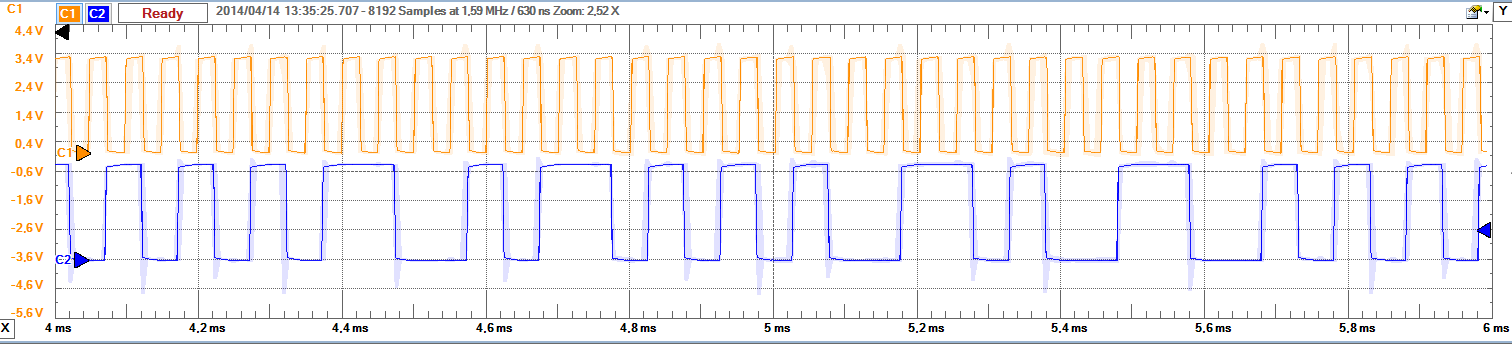
\includegraphics[width=1\textwidth]{billeder/12projectresults/cdr}
	\caption{Clock and data recovery scope picture}
	\label{pic:cdr}
\end{figure}

\section{Custom power line communication bus}
The cusom power line communication bus has been fully implemented on the CDU and the sensor nodes. Two-way communication has been achieved with multiple slaves connected with one wire through the sensors. On figure \ref{pic:trans} is shown a picture of a successful transmission sequence captured by a logic analyser. The transmission is captured on the sensor node and shows the incoming data, the recovered clock and the respond data. In the picture the CDU has requested GetInfo with the function code 1 on address 1. The sensor node responds with the address, the requested function code, no errors and the switch input states.
\begin{figure}[H]
	\centering
	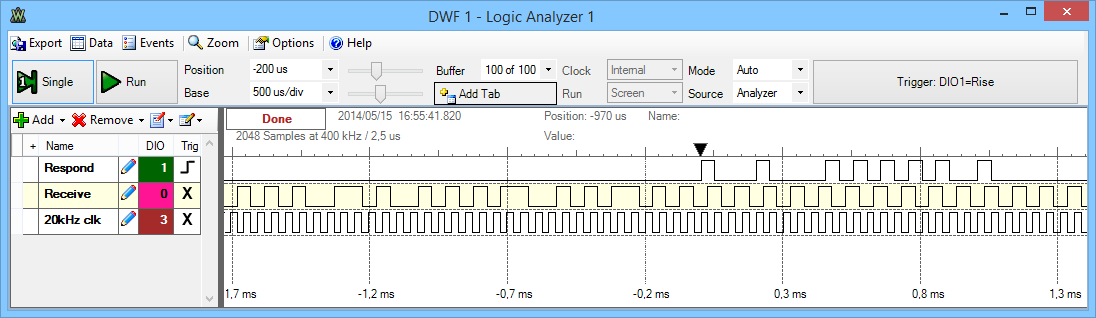
\includegraphics[width=1\textwidth]{billeder/12projectresults/transmission}
	\caption{Logic analyser picture of a successful transmission sequence}
	\label{pic:trans}
\end{figure}

\section{Test results}
The tests in this project provided a baseline for improving the system. The reliability test result showed that less than 1 in 7200 transmissions resulted in an error. The integration tests in the internal test document are all done on the first iteration of the protocol. 



